\documentclass[useAMS,usenatbib]{mn2e}
\usepackage{float}
\usepackage{amsmath}
\usepackage{amssymb}
\usepackage{graphics}
\usepackage{graphicx}
\usepackage{epsfig}
\usepackage{hyperref}
\def\be{\begin{equation}}
\def\ee{\end{equation}}
\def\ba{\begin{eqnarray}}
\def\ea{\end{eqnarray}}

% To highlight comments
\usepackage{color}
\definecolor{red}{rgb}{1,0.0,0.0}
\newcommand{\red}{\color{red}}
\definecolor{blue}{rgb}{0.1,0.3,0.9}
\newcommand{\blue}{\color{blue}}

\usepackage[normalem]{ulem}
\definecolor{darkgreen}{rgb}{0.0,0.5,0.0}

\newcommand{\documentname}{paper~}
\newcommand{\LCDM}{$\Lambda$CDM~}
\newcommand{\beq}{\begin{eqnarray}}
\newcommand{\eeq}{\end{eqnarray}}
\newcommand{\zz}{$z\sim 3$}

\newcommand{\apj}{ApJ}
\newcommand{\apjs}{ApJS}
\newcommand{\apjl}{ApJL}
\newcommand{\aj}{AJ}
\newcommand{\mnras}{MNRAS}
\newcommand{\mnrassub}{MNRAS accepted}
\newcommand{\aap}{A\&A}
\newcommand{\aaps}{A\&AS}
\newcommand{\araa}{ARA\&A}
\newcommand{\nat}{Nature}
\newcommand{\physrep}{PhR}
\newcommand{\pasp}{PASP}
\newcommand{\pasj}{PASJ}
\newcommand{\avg}[1]{\langle{#1}\rangle}
\newcommand{\ly}{{\ifmmode{{\rm Ly}\alpha}\else{Ly$\alpha$}\fi}}
\newcommand{\hMpc}{{\ifmmode{h^{-1}{\rm Mpc}}\else{$h^{-1}$Mpc }\fi}}
\newcommand{\hGpc}{{\ifmmode{h^{-1}{\rm Gpc}}\else{$h^{-1}$Gpc }\fi}}
\newcommand{\hmpc}{{\ifmmode{h^{-1}{\rm Mpc}}\else{$h^{-1}$Mpc }\fi}}
\newcommand{\hkpc}{{\ifmmode{h^{-1}{\rm kpc}}\else{$h^{-1}$kpc }\fi}}
\newcommand{\hMsun}{{\ifmmode{h^{-1}{\rm
        {M_{\odot}}}}\else{$h^{-1}{\rm{M_{\odot}}}$~}\fi}}
\newcommand{\hmsun}{{\ifmmode{h^{-1}{\rm
        {M_{\odot}}}}\else{$h^{-1}{\rm{M_{\odot}}}$}\fi}}
\newcommand{\Msun}{{\ifmmode{{\rm {M_{\odot}}}}\else{${\rm{M_{\odot}}}$}\fi}}
\newcommand{\msun}{{\ifmmode{{\rm {M_{\odot}}}}\else{${\rm{M_{\odot}}}$}\fi}}
\newcommand{\lya}{{Lyman$\alpha$~}}
\newcommand{\clara}{{\texttt{CLARA}}~}
\newcommand{\rand}{{\ifmmode{{\mathcal{R}}}\else{${\mathcal{R}}$ }\fi}}
\newcommand{\hs}{{\hspace{1mm}}}
\newcommand{\muavg}{\vert\langle\cos\theta\rangle\vert}
% definition to produce a "less than or similar to" symbol
\def\lsim{~\rlap{$<$}{\lower 1.0ex\hbox{$\sim$}}}

% definition to produce a "greater than or similar to" symbol
\def\gsim{~\rlap{$>$}{\lower 1.0ex\hbox{$\sim$}}}

\begin{document}

\title[A new method for concentrations]{A new method to estimate
  dark matter halo concentrations}
\author[Poveda \& Forero-Romero]{
\parbox[t]{\textwidth}{\raggedright
  Christian Poveda$^{1}$ \&
  Jaime E. Forero-Romero$^{1}$
}
\vspace*{6pt}\\
$^{1}$Departamento de F\'{i}sica, Universidad de los Andes, Cra. 1
No. 18A-10, Edificio Ip, Bogot\'a, Colombia\\
}
\maketitle

\begin{abstract}
asd
\end{abstract}
\begin{keywords}
methods: numerical, galaxies: haloes, cosmology: theory, dark
matter
\end{keywords}


\section{Introduction}
\label{sec:introduction}
In the concordance cosmology paradigm the the matter content of the
Universe is dominated by dark matter which behaves as a collisionless
fluid under the influence of gravity. In the last three decades
numerical experiments have made possible the simulation of dark matter
dominated universes, yielding valuable insights on the large scale
structure formation process as depicted in observations.

One of the most striking results of these simulations is that dark
matter clumps on galactic scales follow a universal density profile
which in a first approximation is spherical symmetric and only
dependent on the radial coordinate. These profiles seem to be
universal; independent of the cosmological parameters and self-similar
for different spatial scapes after an addecuate re-scaling is
appplied.

One the most commong parameterization of this density is known as the
Navarro-Frenk-White (NFW) profile \citep{NFW}. This profile is a
double power law in radius, where the transition between the two
happens at the so-called scale radius $r_s$. The ratio between the
scale radius and the virial radius of the halo $R_v$ is known as the
concentration $c=R_V/r_s$, a quantity that has been found to be
correlated with the halo mass.

The relationship between halo mass and concentration is in principle
accesible to observations and provides a potential test of LCDM on
galactic scales. With this promise a great deal of effort has been
invested in calibrating this relationship with simulations but also
finding the best possible way to constraint it with observations.

From the computational point of view there are two main methods to
estimate the concetration parameter of a dark matter halo in a N-body
simulation. The first method takes the particles comprosing the halos
and bins them in logarithmic radii to estimate the density in each
bin, then it proceeds with a fit of this density estimation as a
function of radius. A second method uses an analytical property of the
NFW that related the maximum of the ratio of the circular velocity to
the virial velocity. In this method at each particle radius this ratio
is estimated to find the maximum value for this ratio; this value is
used to find the roots of an equation which represent the
concentration parameter.

The first method although is straightforward to apply has two main
disadvantages. First of all it requires a large number of particles in
order to have a proper density estimate in each bin. For a very low
number of particles is hard to define a large number of bins to
proceed with the fit. The second problem is that, as in any process
involving data binning, there is not an way to estimate the optimal
bin size, which in turn can affect the results of the fit.

The second method solves the two problems mentioned above. It works
with low particles numbers and does not involve data binning. However,
it effectively takes into account a single data point and discards the
behaviour of the ratio $V_{cirv}/V_{vir}$ below and above its
maxima.

In this paper we propose a new method to estimate the dark matter halo
concentration from N-body simulation results. This method has two
advantages with respect to the methods mentioned above. First, it does
not involve data binning. Second, it does not throw away data
points. Third, it allows for an straightforward estimation of the
uncertainties in the concentration parameter.

Our method consists in building the cumulative mass profile from the
particle data in the N-body simulation to find the best possible
concentration value using a Markov Chain Monte Carlo methodology by
comparing the data against the analytical expectation.

This paper is structured as follows. In Section \ref{sec:basics} we
review the basic properties of the NFW density profile and define the
basic notation for the rest of the paper. Next in Section
\ref{sec:method} we present our new method to estimate the halo
concentration, payin special attention to the bayesian framework to
find the most probable value and its uncertaintt. In Section
\ref{sec:halo_sample} we demonstrate the power of our method with two
different halo samples; the first one generated under controlled
conditions and the second taken from a cosmological N-body
simulation. Next in \ref{sec:discussion} we discuss these results by
comparing them against other methods to estimate the concentration and
comment on the consequences for the concentration-mass
relationship. We present our conclusions in Section \ref{sec:conclusions}.



\section{Basic properties of the NFW density profile}
\label{sec:basics}

\subsection{Density profile}

The NFW density profile can be written as

\begin{equation}
\rho(r) = \frac{\rho_c\delta_c}{r/r_s(1+r/r_s)^2},
\label{eq:definition}
\end{equation}
%
where $\rho_c\equiv 3H^2/8\pi G$ is the Universe critical density,
$\delta_c$ is the halo dimensionless characteristic density and $r_s$
is known as the scale radius, the radius that marks the transition
between the power law scaling $\rho\propto r^{-1}$ for
$r<r_s$ and $\rho\propto r^{-3}$ for  $r>r_s$.

We define the virial radius of a halo, $r_v$, as the boundary of the
spherical volume that encloses a density of $\Delta_h$ times
the average density of the Universe. The corresponding mass $M_{v}$,
the virial mass, can be written as $M_{v} =
\frac{4\pi}{3}\bar{\rho}\Delta_h r_v^3$.


\subsection{Integrated Mass}
From these definitions we can compute the total mass enclosed inside a
radius $r$:
\begin{equation}
M(<r) = 4\pi\rho_c\delta_c  r_s^3\left[\ln \left
  (\frac{r_s+r}{r}\right) - \frac{r}{r_s+r}\right].
\end{equation}

We express the same quantity in terms of dimensionless
variables $x\equiv r/r_v$ and $m\equiv M(<r)/M_v$,
%
\begin{equation}
m(<x) =
\frac{1}{A}\left[\ln\left(1+xc\right)-\left(\frac{xc}{xc+1}\right)\right],
\label{eq:profile}
\end{equation}
%
where
%
\begin{equation}
A=\ln\left(1+c\right)-\left(\frac{c}{c+1}\right),
\end{equation}
%
and the parameter $c$ is known as the concentration $c\equiv r_v/r_s$.

From this normalization value and for later convenience we define the
following function
%
\begin{equation}
f(x) = \ln\left(1+x\right)-\left(\frac{x}{x+1}\right).
\label{eq:f_NFW}
\end{equation}
%

The most interesting feature of Eq. (\ref{eq:profile}) is that the
concentration is the only free parameter to describe the density
profile. In Figure \ref{fig:profiles} we show $m(<x)$ as
a function of $x$ for different values of the concentration in the range
$1\leq c \leq 20$.

\begin{figure}
\begin{center}
  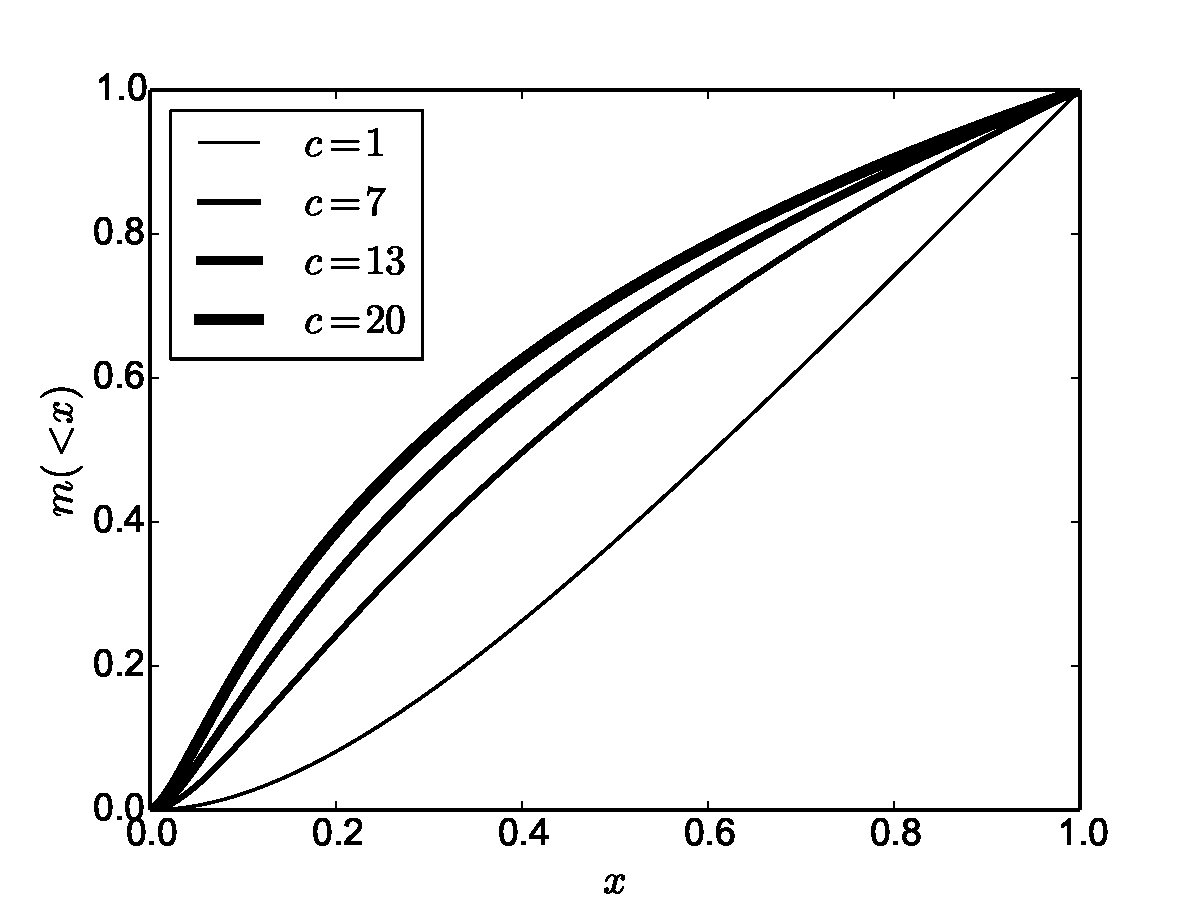
\includegraphics[width=0.48\textwidth]{nfw_normalized.pdf}
\end{center}
\caption{Dimensionless mass profiles as a function of the
  dimensionless radius for different concentration values.
    \label{fig:profiles}}
\end{figure}

\subsection{Circular velocity}

It is also customary to express the mass of the halo in terms of the
circular velocity $V_{c}=\sqrt{GM(<r)/r}$. From this we can
define a new dimensionless circular velocity $v(<x)\equiv
V_{c}(<r)/V_{c}(<r_v)$, using the result in Eq. \ref{eq:profile}
to have:


In Figure \ref{fig:velocity} we show the circular velocity profile for the same
concentrations as in Figure \ref{fig:profiles}.

\begin{equation}
v(<x)=\sqrt{\frac{1}{A}\left[\frac{\ln\left(1+xc\right)}{x}-\frac{c}{xc+1}\right]},
\end{equation}
%
this normalized profile always shows a maximum provided that the
concentration is larger than a values of $c>???$.
It is possible to show that for the NFW profile the maximum is
provided by

\begin{equation}
\mathrm{max}(v(<x)) = \sqrt{\frac{c}{x_{\rm max}}\frac{f(x_{\rm
      max})}{f(c)}},
\label{eq:max_v}
\end{equation}
where $x_{\rm max}=2.163$ and the function $f(x)$ was defined in Eq. (\ref{eq:f_NFW}).

\begin{figure}
\begin{center}
  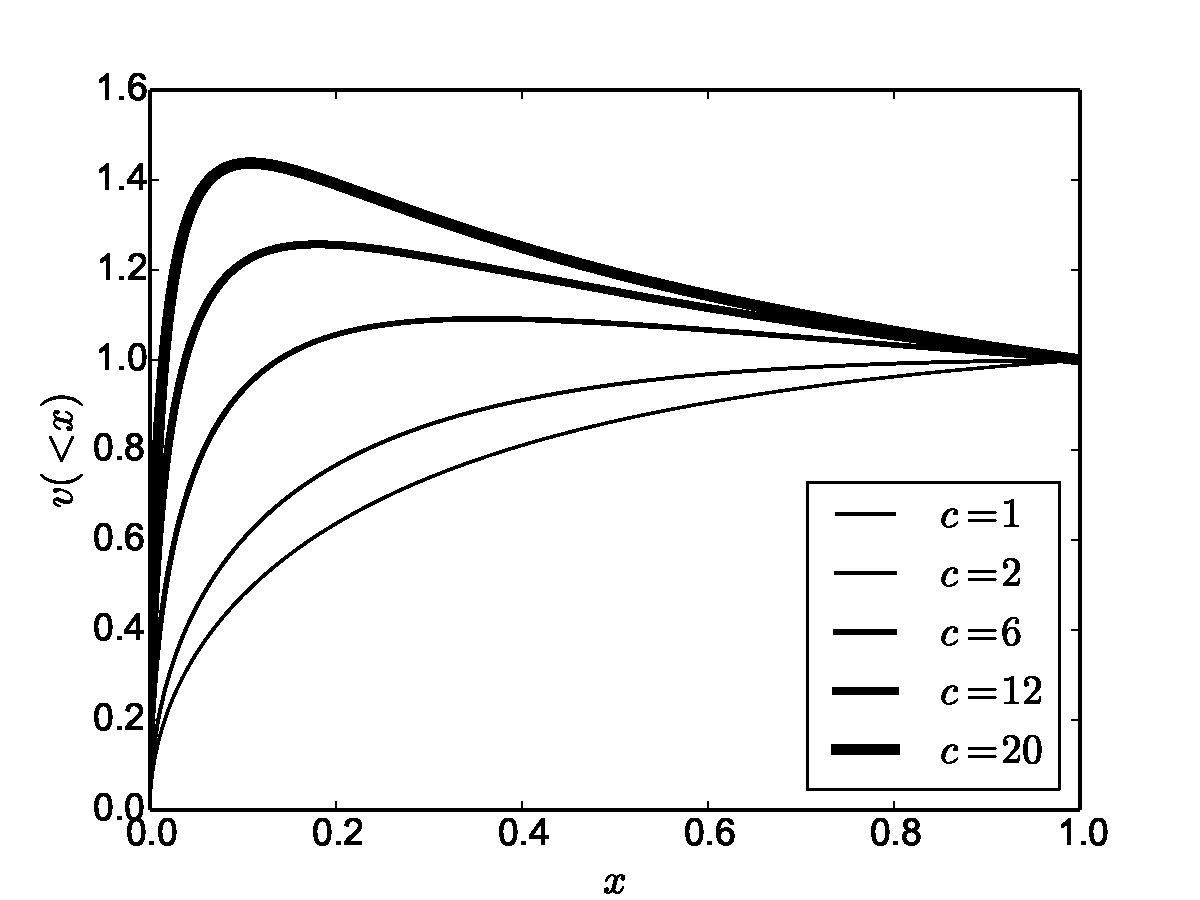
\includegraphics[width=0.48\textwidth]{vel_normalized.pdf}
\end{center}
\caption{Dimensionless velocity profiles as a function of the
  dimensionless radius for different concentration values.
    \label{fig:velocity}}
\end{figure}

\section{A new approach to estimate the halo concentration}
\label{sec:method}

As we saw in the previous sections, once the density profile is
expressed in dimensionless variables the only free parameter in the
density profile  is the concentration. There are two main methods to
estimate concentrations in dark matter halos extracted from N-body
simulations.

The first method tries to directly estimate the density profile.
It takes all the particles in the halo and bins them in the logarithm
of the radial coordinate from the halo center.
Then, it estimates the density in each logarithmic bin counting the
particles and divinding by the corresponding shell volume.
At this point is is possible to make a direct fit to the density as a
function of the radial coordinate.
This method has been most recently used by \cite{Ludlow2014} to study
the mass-concentration-redshift relation of dark matter halos using
the Millennium Simulation Series.

A second method uses the circular velocity profile.
As it was shown in Fig. (\ref{fig:velocity}) the circular velocity
shows a maximum for all profiles with concentration values larger than
$c>2$.
The method finds the value of $x$ for which the normalized circular
velocity $v(<x)$ shows a maximum.
Using this value it solves numerically for the corresponding value of
the concentration using Eq. (\ref{eq:max_v}).
This method has been most recently used by \cite{Klypin2014} to study
the mass-concentration-redshift relation using the Multidark
Simulation Suite.

Our method is a third option that uses the integrated mass profile.
First we define the center of the halo to be at the position of the
particle with the lowest gravitational potential.
Then we rank the particles by their increasing radial distance from
the center.
From this ranked list of $i=1,N$ particles, the total mass at a radius
$r_i$ is $M_i=i\times m_p$, where $r_i$ is
the position of the $i$-th particle and $m_p$ is the mass of a single
computational particle.
In this process we discard the particle at the center.

We stop the construction of the integrated mass profile once we arrive
at an average density of $\Delta_h\bar{\rho}$, with $\Delta_h=740$,
roughly corresponding to 200 times the critical density.
This radius marks the virial radius and the virial mass.
We divide the enclosed mass mass $M_i$ and the radii $r_i$ by these
virial values to obtain the dimensionless variables $m_i$ and $x_i$.

The construction of the numerical integrated mass profile has the
advantage that it does not involve any binning and uses the
information from all the particles in the halo, unlike the method that
tries to directly build.
Furthermore, as it will be clear in the next paragraph, the fit of
this computational profile to the analytic expectation uses the
information from all points, not only a single maxima point as the
method using the circular velocity profile.

We use a Metropolis-Hastings algorithm to sample the likelihood
function distribution defined by ${\cal L}(c)=\exp(-\chi^2(c)/2)$
where the $\chi^2(c)$ is written as

\begin{equation}
\chi^2(c)= \sum_{i=1}^{N}[\log m_i - \log m(< x_i;c)]^2,
\end{equation}
%
where $m(<x_i;c)$ corresponds to the values in Eq.(\ref{eq:profile}) at
$x=x_i$ for a given value of the concentration parameter $c$ and the
$i$ index sums over all the particles in the numerical profile.

For the walk in the Metropolis-Hastings algorithm we used 50000 steps
where each step was randomly generated with a normal distribution
centered around the last step with an standard deviation of
$\sigma=0.03$.
From the $\chi^2$ distribution we find the optimal value of the
concentration and  its associated uncertainty.

\section{Results}
\label{sec:results}

In this Section we present the results of applying our method on two
different halo samples.

The first sample is composed by mock halos generated to have known
concentration values in perfect spherical symmetry following an NFW
profile.
We use this sample to check that we can recover the expected values
but also gauge the impact of the number of particles on the outcomes
and the difference with respect to the two other fitting methods.


The second sample comes from a publicly available N-body cosmological
simulation.
From this sample we quantify again the differences between all the
methods we have to fit the data.
We also estimate the possible impact of the different methods in
estimating the mass-concentration relationship from simulations.

\subsection{Tests on Mock Halos}

The method we use to generate the halos is based on the integrated
mass profile.
We start by fixing the desired concentration $c$ and total number of
particles $N$ in the mock halo
With this values we define the mass element as $\delta m = 1/M$, corresponding
to the mass of each particle such that the total mass is one.
Then for each particle $i=1,\ldots,N$, we find the value of $r_i$ such that
the difference
%
\begin{equation}
m(<r_i;c) - i \cdot \delta m
\end{equation}
%
is zero using Ridders' method.

The value of $r_i$ is the radius of the $i$-th particle of the mock
halo.
Then we generate random polar and azimuthal angles $\theta$ and $\phi$
for each particle to ensure spherical symmetry.
Finally these three spherical coordinates are transformed into cartesian coordinates
$(r,\theta,\phi) \rightarrow (x,y,z)$.



We generate in total $400$ mock halos splitted into four different
groups of $100$ halos each.
The four groups differ in the total number of particles for their halos:
$20$, $200$, $2000$ and $20000$.
Inside each group the halos have random concentration values in
the range $1<c<20$ with a flat distribution.
For all these halos with find the concentration values using the
density, velocity and mass methods described in the previous
section. We quantify the difference between the expected $c_{in}$
and obtained $c_{out}$ values by

\begin{equation}
D=(c_{in}-c_{out})/c_{in}.
\label{eq:D}
\end{equation}

\subsubsection{The impact of particle number}

\begin{figure}
\begin{center}
  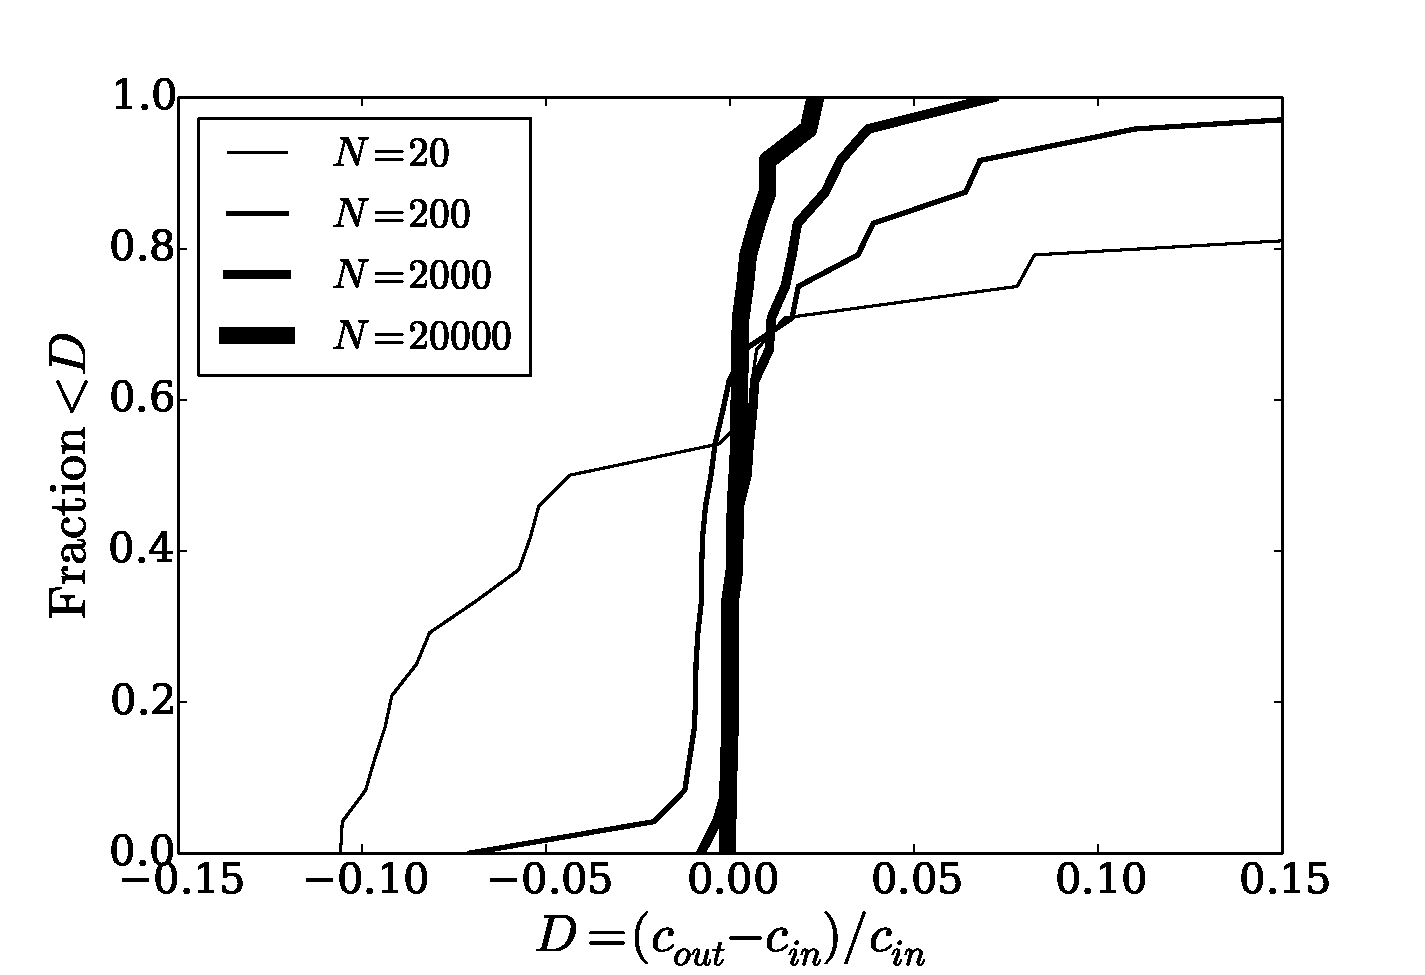
\includegraphics[width=0.50\textwidth]{percentual_diff.pdf}
\end{center}
\caption{Cumulative distribution of the fractional difference, $D$, between
  the input concentration in the mock halo generator, $c_{in}$ and the
  measurement by our MCMC code, $c_{out}$. Each curve corresponds to
  halos generated with a different number of particles, $N$.
    \label{fig:results_mocks}}
\end{figure}

Figure \ref{fig:results_mocks} shows the integrated distribution for
$D$ for the fits using our method, splitted into four different groups
according the particle number.
From this Figure the first immediate
conclusion is that increasing the number of particles increases the
chances to recover the input values.

We believe that the main effect that contributes to this trend
is that the particle that our algorithm finds to be the halo center
(where the potential is minimum) gets closer to the original
geometrical center (where no particle sits by construction) used to
generate the halo.  Poissonian noise makes this center fluctuate,
changing the numerical radial profile from the analytical input.

For particle number of $20$ the offset betwen the input and output
concentration can be as large as $20\%$, with a slight bias around
$-0.05\%$, i.e. the output concentration is biased towards lower
values than the input.
For particle numbers of $2000$ most of the offsets fall below $5\%$,
with a clear peak around $0\%$ indicating that any appreciable bias is
absent.


\subsubsection{The impact of the input concentration}

{\bf Hace falta hacer una figura para este caso.}

\subsubsection{The impact of different methods}

\begin{figure}
\begin{center}
  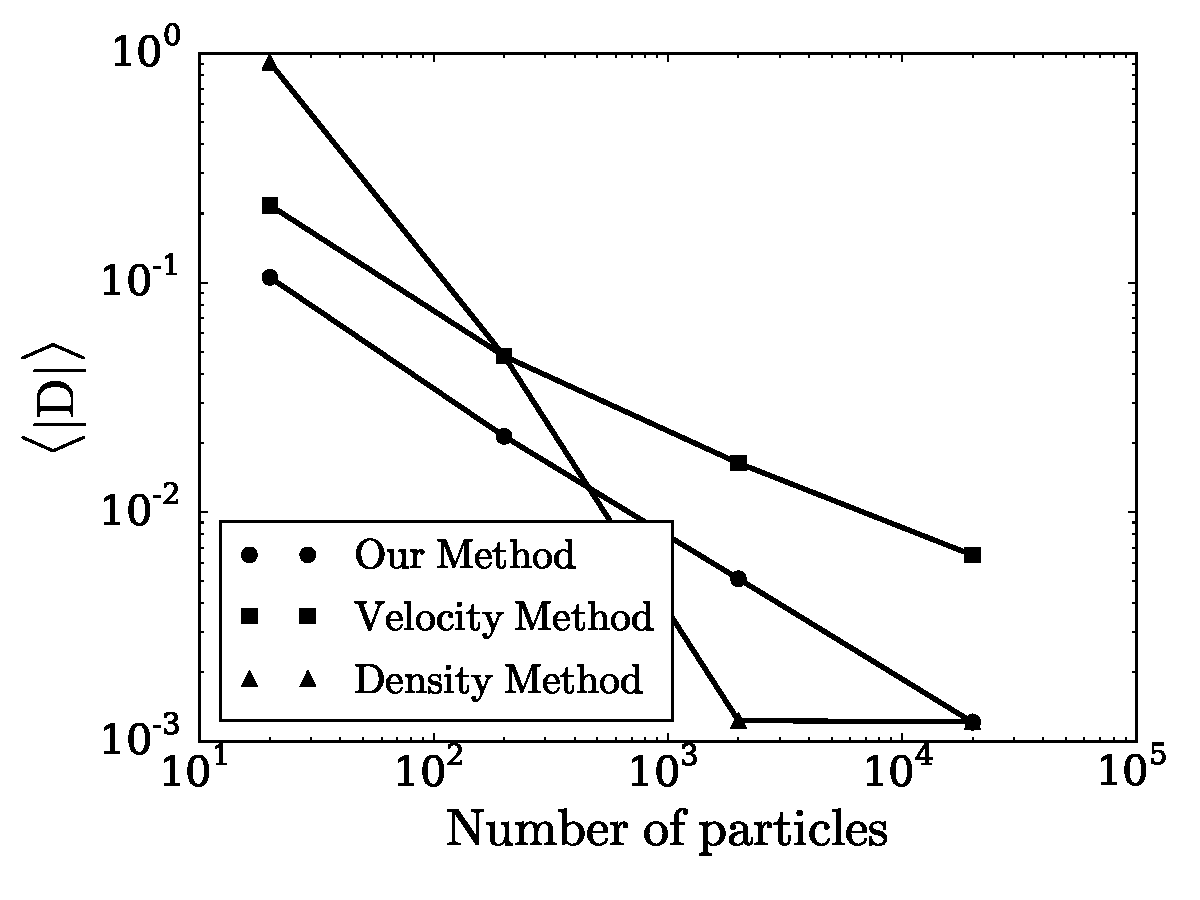
\includegraphics[width=0.48\textwidth]{error.pdf}
\end{center}
\caption{Average value of the relative error in the concentration
  estimate, $\avg{|D|}$, as a function of the particle number $N$ in
  the set of mock halos. Different symbols represent different
  methods. Our method provide the most accurate estimate at fixed
  particle number $N$.
    \label{fig:error}}
\end{figure}


Using this dataset we also compare our method against the other two
methods described earlier: using shells to estimate the density as a
function of radius and the maximum circular velocity method.
In the first case we use the same Metropolis-Hastings algorithm we
have in our methot to fit the density profile.
In the second method we simply follow the procedure described in
Section \ref{sec:method}

We quantify the accuracy of each method with the following statistic:

\begin{equation}
\avg{|D|}=\frac{1}{\left|{\cal{H}}_N\right|}\sum_{{\cal{H}}_N} |D|,
\end{equation}

where ${\cal{H}}_N$ corresponds to the set of haloes with $N$
particles, $D$ follows the definition in Eq. (\ref{eq:D}) and
$\left|{\cal{H}}_n\right|$ is the number of haloes in ${\cal{H}}_n$.


Figure \ref{fig:error} shows the behaviour of $\avg{|D|}$ as a function of
halo particle number for the three different methods to estimate the
concentration.
At fixed particle numbers our method always shows the lowest
$\avg{|D|}$ values compared to the other two methods.
Its accuracy is on the order of $10\%$ for $20$ particles in the halo,
going down to $0.1\%$ for halos with $20000$ particles.
The decrease of $\avg{|D|}$ with increasing particle number $N$ goes
approximately as $\avg{|D|}\propto N^{-1/2}$, which reinforces the hint that
the accuracy of the method is related to a decrease of Poissonian
noise.

The second best accuracy is achieved by the method based on the
maximum of the circular velocity.
It also shows a similar behaviour $\avg{|D|}\propto N^{-1/2}$.
Its accuracy is $2-5$ times less than in our method, on the order of
$20\%$ for $20$ particle halos and $0.5\%$ for $20000$ particle halos.
The method based on the direct density fit shows the lowest accuracy
of all methods.
Its average values $\avg{|D|}$ are always between $30\%$ adn $50\%$
regardless of the particle number. {\bf Necesitamos entender el
  comportamiento de esto.}

\subsection{Tests on N-body data}
\label{sec:data}
\begin{figure}
  \begin{center}
    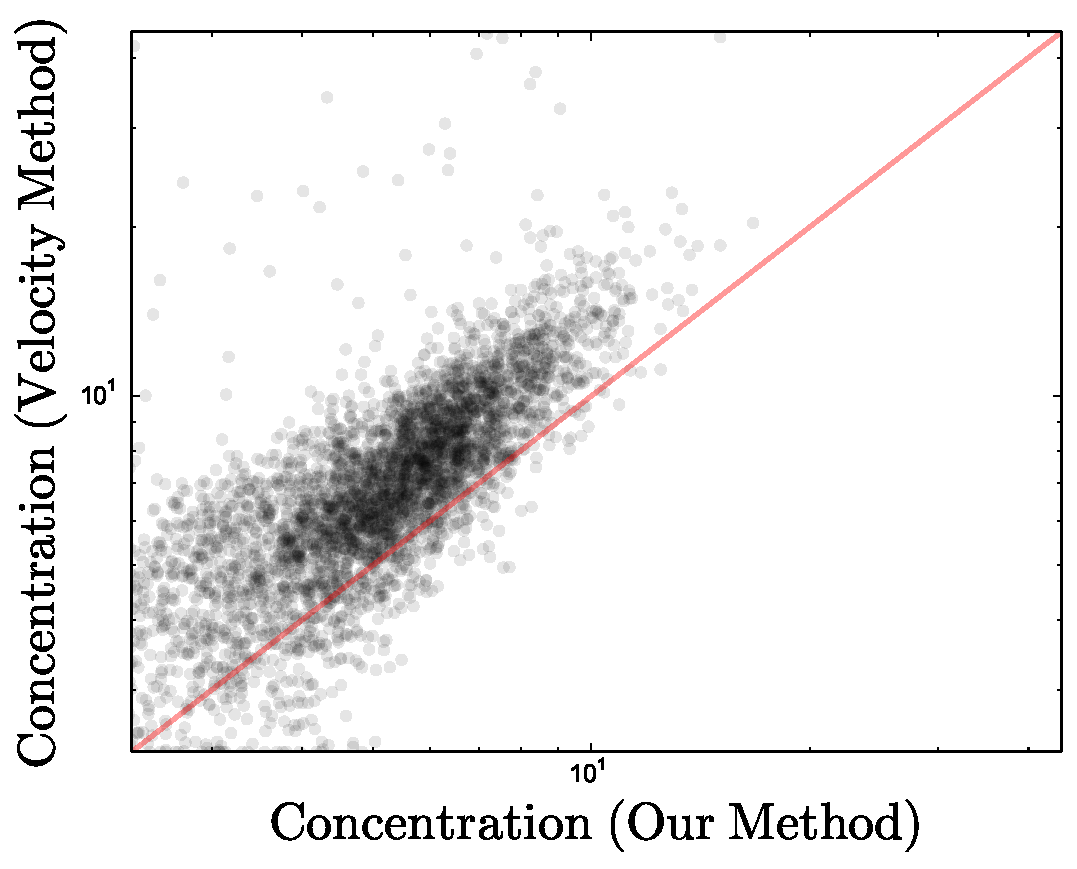
\includegraphics[width=0.48\textwidth]{mass-velocity.pdf}
  \end{center}
  \caption{Comparison between the obtained concentrations by our method and the velocity method
  \label{fig:mdv}}
\end{figure}

\begin{figure}
  \begin{center}
    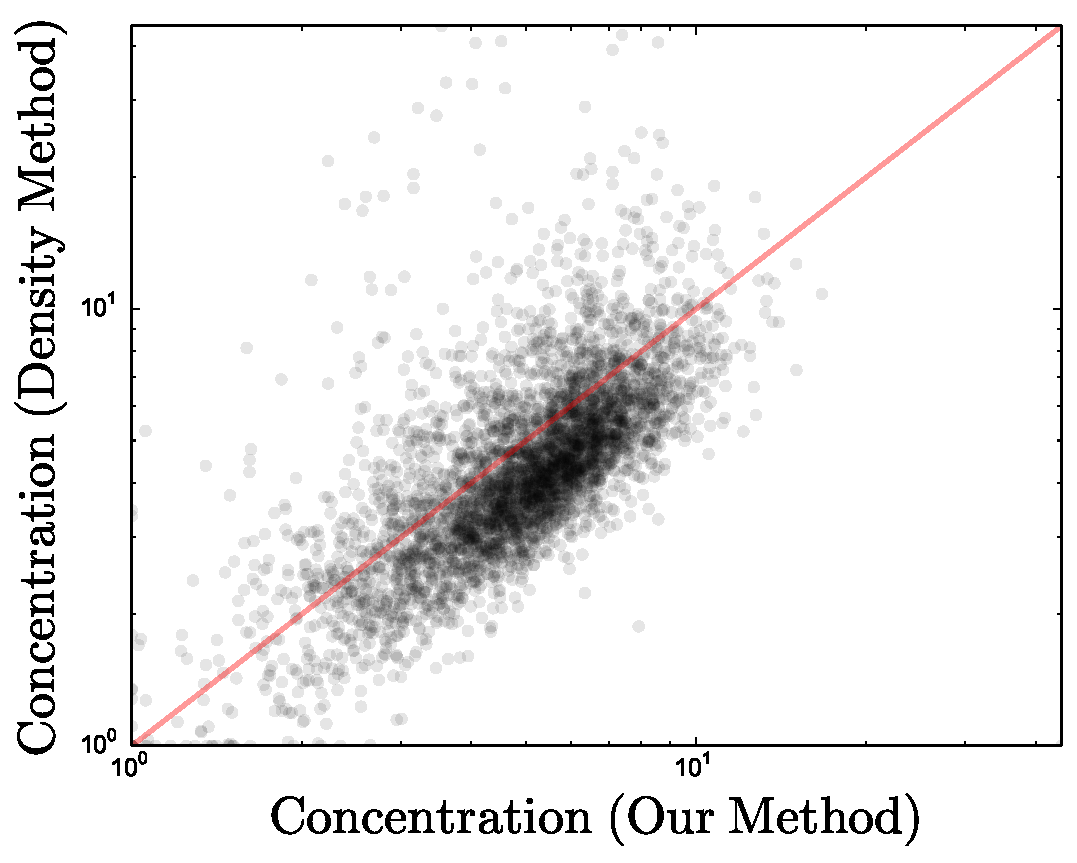
\includegraphics[width=0.48\textwidth]{mass-density.pdf}
  \end{center}
  \caption{Comparison between the obtained concentrations by our method and the density method
  \label{fig:mdv}}
\end{figure}

\begin{figure}
  \begin{center}
    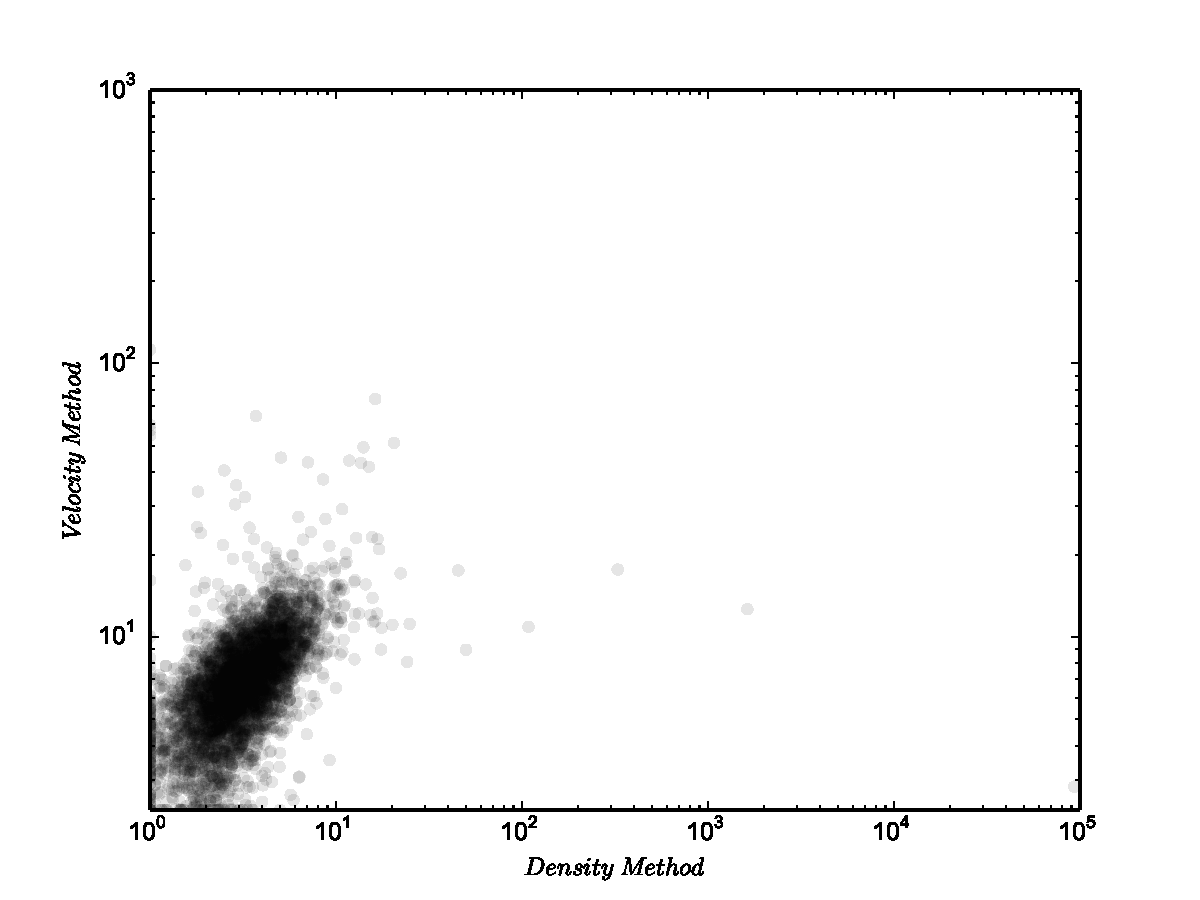
\includegraphics[width=0.48\textwidth]{density-velocity.pdf}
  \end{center}
  \caption{Comparison between the obtained concentrations by the density method and the velocity method
  \label{fig:mdv}}
\end{figure}

\begin{figure*}
\begin{center}
  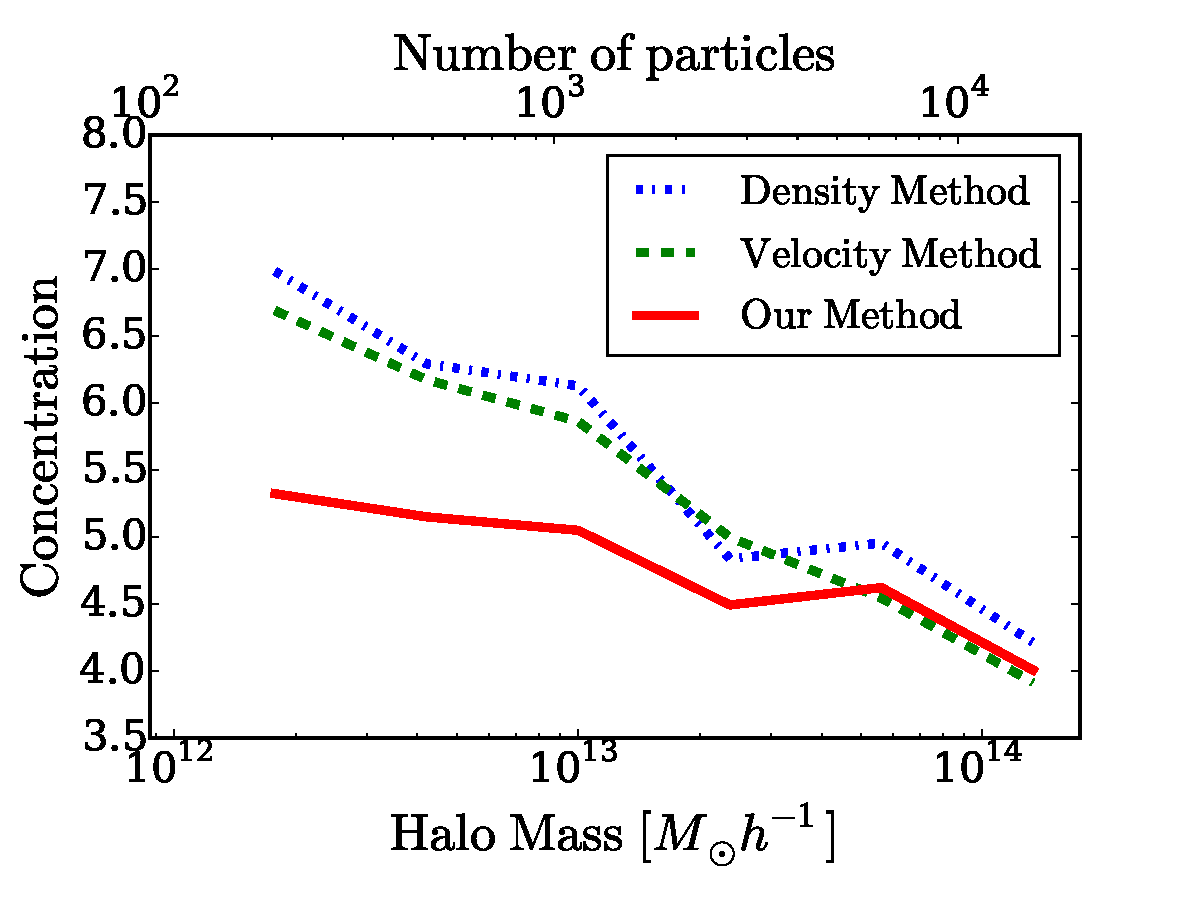
\includegraphics[width=0.90\textwidth]{concentration.pdf}
\end{center}
\caption{Mass-concentration relationship for the three different
  methods used on the same cosmological N-body data. The central lines
  correspond the median and the shadowed region indicates the
  quartiles.
    \label{fig:concentrations}}
\end{figure*}



We use data from the MultiDark cosmological simulation.
It follows the non-linear evolution of a dark matter density field
sampled with $2048^3$ particles over a cubic box of $1000$ \hMpc on a side.
The data is publicly available through \url{http://www.cosmosim.org/}.
More details about the structure of the database and the simulation
can be found in \citep{2013AN....334..691R}.

We build a sample of all halos located in a cubic sub-volume of $100$
\hMpc on a side centered on the most massive halo in the simulation at
$z=0$ which corresponds to the \texttt{miniMDR1} tables in the
database.
From this sample we select all the halos at $z=0$ detected with a
Friends-of-Friends (FoF) algorithm with masses in the interval
$10^{11}\leq M_{\rm FoF}/\hMsun \leq 10^{15}$.
The FoF algorithm used with a linking length of $0.17$ times the average
interparticle distance. This choice translates into an overdensity
$\Delta_h\sim 400-700$ dependent on the halo concentration
\citep{More2011}.
Finally, for each FoF halo we select from all the particles that
belong to it.

From this set of particles we follow the procedure spelled out in
Section \ref{sec:method} with $\Delta_h=740$  (corresponding to $200$
times the critical density) to find the halo concentration.
This choice makes that our overdensities are fully included inside the
original FoF particle group.
We only report results from overdensities with at least $100$ particles.
Finally, we store the values obtained for the virial radius, virial
mass and concentration.


Figure \ref{fig:mdv} shows the results that compare the concentration
values in the simulated halos from the three different methods.
At zeroth order the results are consistent.
However, the concentration values from the velocity method produces
concentrations that are $XXX$ times larger on average than the results
from our method.
On the other hand, the concentrations from the velocity method are
$XXX$ times lower than in our method.

%Running another test with halos whose concentrations vary as a normal
%distribution of variance ${\sigma}^2$ we found that the concentrations
%obtained by the method of circular velocity are a 35\% greater than
%the ones obtained by the density method. However the concentrations
%obtained by the velocity method are barey higher (around 2\% or 3\%)
%than the ones obtained by our method. We did not find any significant
%variation in the concentration values obtained by any method by
%changing ${\sigma}^2$ in contrast with FIXME.


Figure \ref{fig:concentration} shows the mass-concentration
relationship from the N-body data with the results of the three
different methods.
The central lines correspond the median and the
shadowed region indicates the quartiles.
In this relationship our methods represents a compromise between the
velocity and density methods.
The slope is flatter and the overall normalization is below the
velocity method and above the density.


\section{Conclusions}
\label{sec:conclusions}


\bibliographystyle{mn2e}
\bibliography{references}

\end{document}
